Neste capítulo mostraremos exemplos de resultados de utilização da ferramenta, para isso demonstraremos com alguns códigos simples a interação com o sistema e seus resultados,

\begin{itemize}
	\item Soma simples
	%\item Sequência de fibonacci
\end{itemize}


\section{Possíveis erros de montagem}

	Como explicado na seção anterior, sendo a montagem, a parte que lida diretamente com a entrada do usuário, é necessário que o sistema saiba lidar com possíveis erros inseridos no código e devolver uma resposta adequada, foram implementados as seguintes menasgens de erros,

	\begin{itemize}
		\item Na figura \ref{fig:assemble_error_duplicated_symbol}, temos um exemplo de erro de declaração múltipla de símbolo, ou seja, se o programador declarar o mesmo símbolo em dois momentos diferentes no código.
		\item Na figura \ref{fig:assemble_error_directives_strings}, temos um exemplo de erro da diretiva .asciiz ou .string, quando é declarado mais de uma string para um único símbolo.
		\item Na figura \ref{fig:assemble_error_imediato}, temos um exemplo de erro de valor de imediato, no caso deste projeto onde utilizamos tamanhos de palavra 32 bits, um valor superior a 4GB traria um overflow.
		\item Na figura \ref{fig:assemble_error_operando_invalido}, temos um exemplo de erro de operando inválido, a instrução ADDI pede um imediato como último argumento, porém é fornecido um registrador.
		\item Nas figuras \ref{fig:assemble_error_operation_not_recognized}, e \ref{fig:assemble_error_op_not_recog_directives}, temos um exemplo de erro de operação não reconhecida, sendo que o primeiro mostra que foi fornecido uma instrução desconhecida, e no segundo uma diretiva desconhecida.
		\item Na figura \ref{fig:assemble_error_simbolo_inexistente}, temos um exemplo de erro de símbolo inexistente, o programador tentou utilizar um símbolo que não foi declarado antes.
		\item Na figura \ref{fig:assemble_error_wrong_arguments}, temos um exemplo de erro de tipo ou número de argumentos de diretiva, parecido com o erro da figura \ref{fig:assemble_error_directives_strings}. Neste exemplo a diretiva .word pede um número e lhe é fornecido outra label.
	\end{itemize}

	\begin{figure}[h]
	  \centering
	  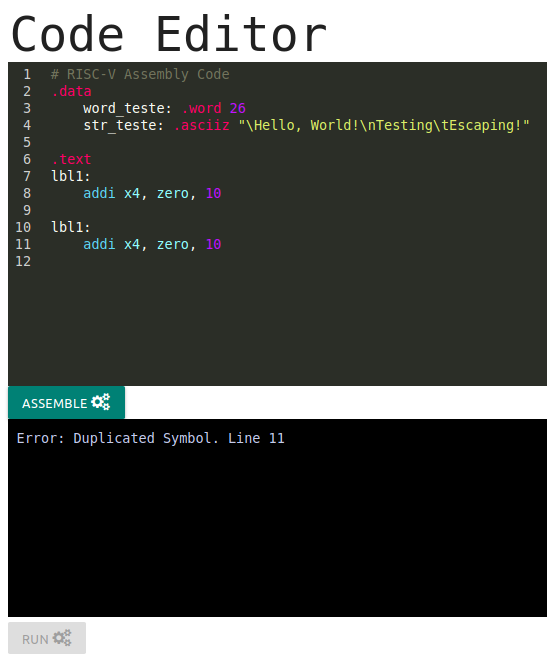
\includegraphics[width=8cm]{img/assemble_error_duplicated_symbol.png}
	  \caption{Erro de declaração múltipla de símbolo.}
	  \label{fig:assemble_error_duplicated_symbol}
	\end{figure}


	\begin{figure}[h]
	  \centering	  
	  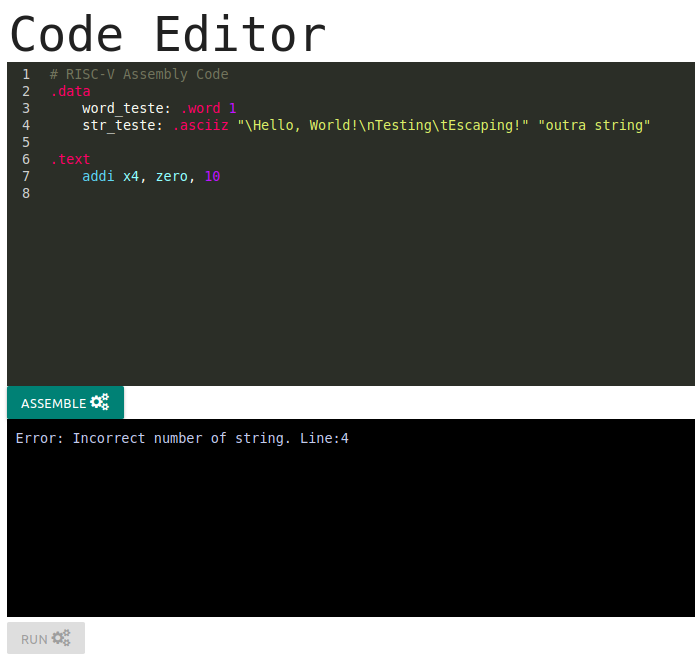
\includegraphics[width=8cm]{img/assemble_error_directives_strings.png}
	  \caption{Erro de declaração de diretiva string.}
	  \label{fig:assemble_error_directives_strings}
	\end{figure}


	\begin{figure}[h]
	  \centering
	  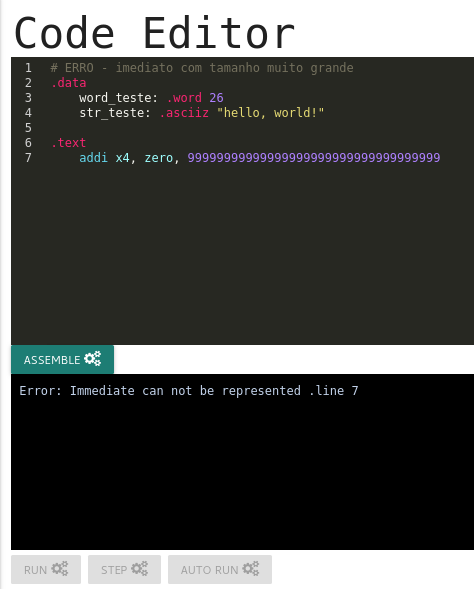
\includegraphics[width=8cm]{img/assemble_error_imediato.png}
	  \caption{Erro de imediato para o tamanho 32 de palavra 32 bits.}
	  \label{fig:assemble_error_imediato}
	\end{figure}

	\begin{figure}[h]
	  \centering
	  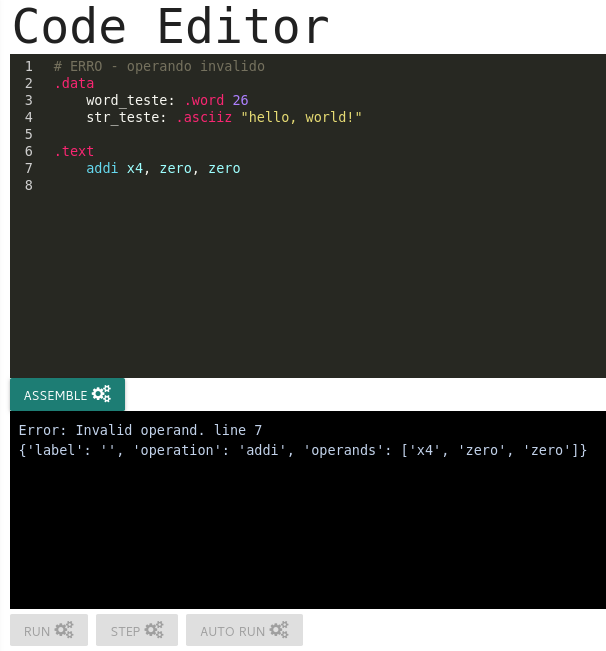
\includegraphics[width=8cm]{img/assemble_error_operando_invalido.png}
	  \caption{Erro de operando inválida, operando de tipo diferente do esperado.}
	  \label{fig:assemble_error_operando_invalido}
	\end{figure}

	\begin{figure}[h]
	  \centering
	  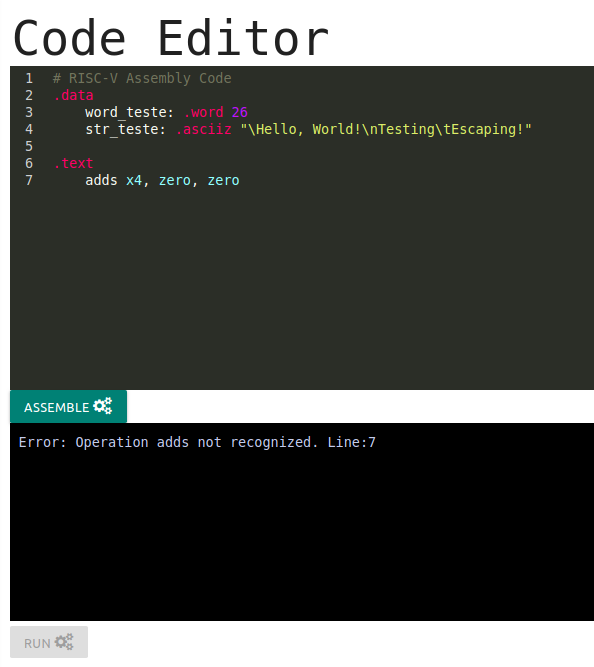
\includegraphics[width=8cm]{img/assemble_error_operation_not_recognized.png}
	  \caption{Erro de operação inválida, instrução não existente na arquitetura implementada.}
	  \label{fig:assemble_error_operation_not_recognized}
	\end{figure}


	\begin{figure}[h]
	  \centering
	  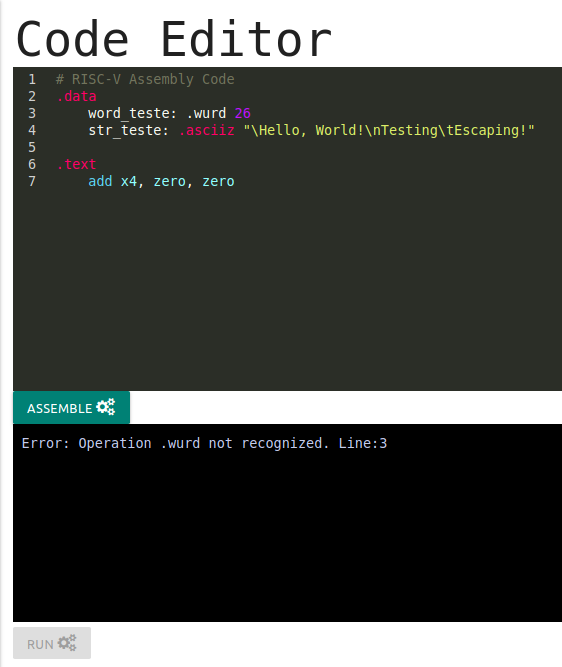
\includegraphics[width=8cm]{img/assemble_error_op_not_recog_directives.png}
	  \caption{Erro de operação inválida, diretiva não existente na arquitetura implementada.}
	  \label{fig:assemble_error_op_not_recog_directives}
	\end{figure}

	\begin{figure}[h]
	  \centering
	  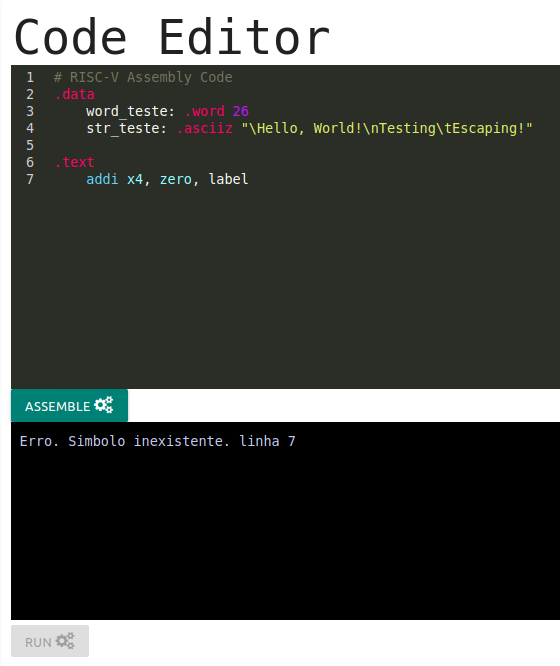
\includegraphics[width=8cm]{img/assemble_error_simbolo_inexistente.png}
	  \caption{Erro de símbolo inválido, símbolo não foi declarado.}
	  \label{fig:assemble_error_simbolo_inexistente}
	\end{figure}

	\begin{figure}[h]
	  \centering
	  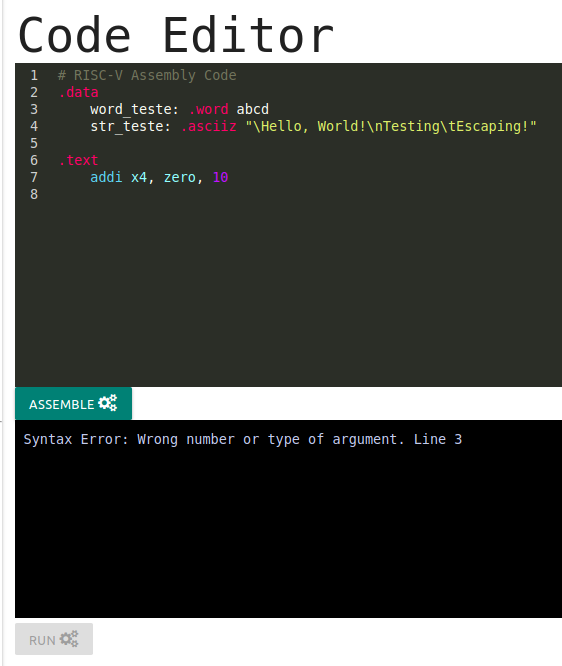
\includegraphics[width=8cm]{img/assemble_error_wrong_arguments.png}
	  \caption{Erro de argumentos de diretiva inválido, o tipo ou número de argumentos está incorreto.}
	  \label{fig:assemble_error_wrong_arguments}
	\end{figure}





\section{Código exemplo}
	exemplos de codigos\\
	imagens\\

\section{Saidas}
	dados de saida\\
	tela de simulação


